\documentclass{article}

\usepackage{multicol}
\usepackage{graphicx}
\usepackage{caption}
\usepackage[left=2cm,right=2cm,top=2cm,bottom=2.5cm]{geometry}

\title{\textbf{MATH 300 Final Project}}
\author{Ali Hamza $|$ Maham Shoaib $|$ Hassan Naseem}
\date{\today}

\begin{document}
\maketitle

\section{Tasks}
\subsection{Task 1}
In this section we made a function $task1(steps,start,leftprob,stopprob)$. The function takes steps using an algorithm that makes use
of an algorithm that can be explained using the following diagram.
\begin{center}
    \includegraphics*[scale = 1]{task1prob.png}
\end{center}
Let us assume
\begin{itemize}
    \item The red region is the probability of not moving
    \item The green region is the probability of moving left
    \item The blue region is the probability of moving right
\end{itemize}
The algorithm simply checks if the randomly generated numbers $0\leq n \leq 1$ lies within a certain 
region and makes movement accordingly.\\\\
Running the algorithm on multiple steps the following graphs were obtained.
%Figure (Images of Graphs Obtained)
    \begin{multicols}{3}[\columnsep=3cm]
        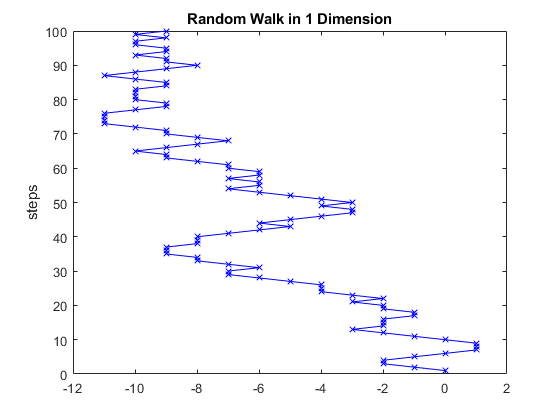
\includegraphics[scale=0.3]{r1d100.png}
        \columnbreak
        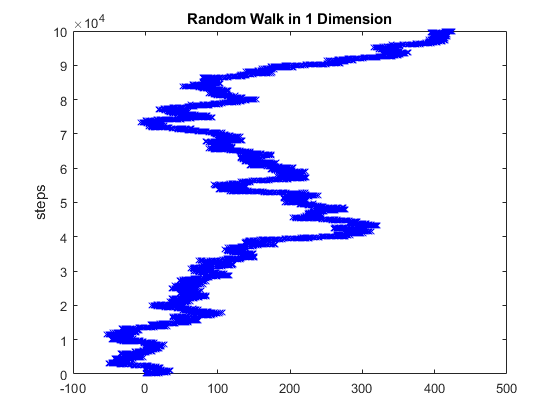
\includegraphics[scale=0.3]{r1d100000.png}%Fix these
        \columnbreak
        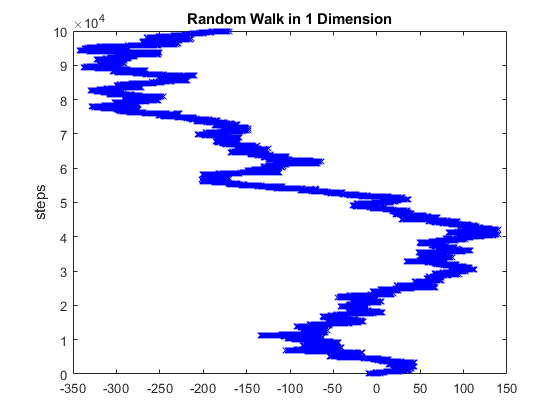
\includegraphics[scale=0.3]{r1d1000000.png}%Fix these 
        \end{multicols}
    \captionof{figure}{Steps = 100, 100000, 1000000 from left to right}
\\\\
To find the expected average distance at a certain step the we ran multiple 
simulations of the code and calculated an average step at each step. This rendered
the following random walk that is made up of average steps. This is then an expected
random walk. 
%include graph here

\subsection{Task 2}
In task 2 we took a similar approach as task 1. The only difference was that we simulated a random walk 
for two particles on the same graph. However, the same issues of randomness arose and it was impossible to
predict the average step at which the two particles met. 
\\\\
Similar, to task 1 we simulated multiple random walks of the two particles and calculated the average step 
at which the particles were meeting for a certain number of steps and distance. The data of each intercepting 
step was recorded into an array and the average was calculated to find an expected intercepting step.
\\\\
We also plotted the average random walks of the the two particles and the result of that was as follows:
It is worth noting, however, that this graph is also subject to change based on different parameters. However, 
it seems to be stable on multiple executions. There is some deviation though. 
%Include graph here
\subsection{Task 3}
\subsection{Task 4}
\subsection{Task 5}

\subsection{Task 6}
\subsection{Task 7}
\subsection{Task 8}
\section{Bibliography}

\end{document}